\documentclass[letterpaper, 10pt, conference]{ieeeconf}
\usepackage{amsmath,amssymb,mathtools,bm}
\usepackage{graphicx}
\usepackage{booktabs}
\usepackage{multirow}
\usepackage{cite}
\usepackage{stfloats}
\usepackage{placeins}
\usepackage[T1]{fontenc}
\usepackage[hidelinks]{hyperref}
\makeatletter
\let\keywords\@IEEESAVECMDkeywords
\let\endkeywords\@IEEESAVECMDendkeywords
\let\PARstart\@IEEESAVECMDPARstart
\makeatother
\hbadness=10000
\vbadness=10000
\setlength{\textfloatsep}{8pt plus 2pt minus 2pt}
\setlength{\floatsep}{10pt plus 2pt minus 2pt}
\setlength{\dbltextfloatsep}{8pt plus 2pt minus 2pt}


\newtheorem{theorem}{Theorem}
\newtheorem{lemma}{Lemma}
\newtheorem{proposition}{Proposition}
\newtheorem{corollary}{Corollary}
\newtheorem{definition}{Definition}
\newtheorem{assumption}{Assumption}
\newtheorem{remark}{Remark}

\newcommand{\E}{\mathbb{E}}
\newcommand{\Prob}{\mathbb{P}}
\newcommand{\R}{\mathbb{R}}
\newcommand{\KL}{\mathrm{KL}}
\newcommand{\dX}{d_{\mathcal{X}}}
\newcommand{\suff}{\mathrm{succ}}
\newcommand{\Afilt}{\mathcal{A}_{\mathrm{filt}}}
\newcommand{\code}[1]{\texttt{#1}}
\newcommand{\esssup}{\mathop{\mathrm{ess\,sup}}}

% Tables below were generated by scripts/paper/make_dataset_table.py and
% make_baseline_table.py and inlined for a standalone submission. Re-run those
% scripts and re-paste if results/rebuttal/*.json changes.
\begin{document}

\title{Learning Manipulation-Sufficient Representations via Outcome
Bottlenecks}

\author{Anonymous Authors}

\markboth{}%
{Anonymous submission: Learning Manipulation-Sufficient Representations}

\maketitle

\begin{abstract}
A robot that offloads perception to a nearby server must decide what to put on the
wire. We ask how few bits a manipulation decision needs, and whether those bits can
carry a guarantee. We formulate perception for manipulation as estimating a calibrated
belief over the minimal statistic that preserves the information which changes action
outcomes, and instantiate it as an action-conditioned stochastic bottleneck: a marginal
outcome log-loss preserves predictive relevance while a rate term controls what is
transmitted. Because the statistic is formed before the action is chosen, one payload
scores every candidate grasp. On 11{,}979 executable simulated grasps over 13 scanned
groceries, an entropy-coded payload of 10 bytes per scene loses nothing measurable
against the fp32 representation, 0.636 against 0.638 within-scene AUC at 0.906 coverage,
a 25-fold reduction. Against a retrained Dex-Net grasp-quality network, whose
representation is formed after the grasp is applied and therefore costs one payload per
candidate, the two methods trace a rate-quality frontier that crosses near 600 bits per
scene: below it our statistic ranks better on eight times fewer bits, above it the
baseline is the stronger ranker. Recalibrating the conformal filter on the selected
action restores the finite-sample guarantee for the grasp actually executed and raises
the certified fraction from 0.372 to 0.510 at 95\% target coverage. Under 20\% packet
loss the system acts on half of all scenes with success unchanged at 0.855, converting
lost payloads into abstentions rather than failed grasps. All results are simulation
only.
\end{abstract}


\IEEEpeerreviewmaketitle

\section{Introduction}

\PARstart{R}{obotic} edge systems often communicate dense geometry optimized
for reconstruction rather than action outcomes~\cite{shi2016edge,%
wen2024foundationpose,fang2020graspnet}. We instead
learn a stochastic interface preserving $p(y\mid o,a)$ for admissible actions.
Outcome log-loss and a KL rate surrogate train one encoder and head used for
selection, filtering, active sensing, and probe updates. Our contributions are:
\begin{enumerate}
\item a decision-sufficient statistic that is formed before the action is chosen, so
one 10-byte payload scores every candidate grasp, measured against a matched
per-action learned representation on a rate-quality frontier;
\item a finite-probe identifiability theorem verified against simulation;
\item a selection-conditional conformal filter whose guarantee covers the grasp the
robot executes rather than a random candidate pair, at a higher certified fraction; and
\item a link study in which packet loss degrades into abstention at constant success,
and a leave-object-out study in which the certificate withdraws rather than misfires.
\end{enumerate}
On 11{,}979 simulated grasps, reconstructed Ferrari--Canny quality reaches
0.542 AUC and falls below chance on curved objects~\cite{ferrari1992planning,%
roa2015grasp}; our 512-byte representation reaches 0.876 AUC and 0.984 success
at 25\% commitment.

\section{Related Work}
\label{sec:related}

Reconstruct-then-plan systems estimate pose, completion, or object-centric
geometry before applying analytic grasp criteria~\cite{wen2024foundationpose,%
ferrari1992planning}. This decomposition is
interpretable but propagates contact-geometry error. Direct grasp networks
predict poses or scores~\cite{mahler2017dexnet,fang2020graspnet}; our method instead exposes a compact
stochastic outcome interface while keeping the action rule separate.
Prior studies show that individual analytic grasp metrics can be weak success
predictors, motivating learned combinations and richer physical labels
~\cite{rubert2017relevance,roa2015grasp,lu2022hybrid}. Our OBB
Ferrari--Canny experiment is therefore a controlled corpus-specific diagnostic,
not a new general indictment of analytic metrics.

The information bottleneck formalizes compression subject to predictive
relevance~\cite{tishby1999,alemi2017}. Existing manipulation variants compress
for a policy or behavior-cloning objective~\cite{pacelli2020,bai2025rethinking};
ours instead preserves the policy-free action-conditioned outcome family.
Task-oriented edge communication also learns rate-controlled IB features, but
for classification rather than supplied-grasp outcome prediction
~\cite{shao2022task,matsubara2022split}. Conformal robotics calibrates planner
constraints or task decisions~\cite{vovk2005,lindemann2023safe}; our layer
calibrates belief-averaged outcome sets and abstains when no success singleton
remains. Table~\ref{tab:positioning} summarizes the resulting intersection.

\begin{table*}[!t]
\centering
\caption{Method positioning. Checkmarks denote design properties, not
cross-paper numerical comparisons. ``Given grasp'' means scoring an externally
supplied candidate rather than only ranking internally generated proposals.}
\label{tab:positioning}
\scriptsize
\setlength{\tabcolsep}{4pt}
\begin{tabular}{llccccc}
\toprule
Family & Representative & Given grasp & No recon. & Rate ctrl. & Calibrated & Abstains \\
\midrule
Reconstruct--plan & FoundationPose~\cite{wen2024foundationpose} & via metric & -- & -- & -- & -- \\
Analytic quality & Ferrari--Canny~\cite{ferrari1992planning} & $\checkmark$ & -- & -- & -- & -- \\
Metric/label learning & Rubert; FGC~\cite{rubert2017relevance,lu2022hybrid} & $\checkmark$ & varies & -- & -- & -- \\
Learned quality & Dex-Net 2.0~\cite{mahler2017dexnet} & $\checkmark$ & $\checkmark$ & -- & -- & -- \\
Manipulation IB & Pacelli; BC-IB~\cite{pacelli2020,bai2025rethinking} & policy-tied & $\checkmark$ & $\checkmark$ & -- & -- \\
Edge IB & VL-VFE~\cite{shao2022task} & -- & $\checkmark$ & $\checkmark$ & -- & -- \\
Conformal robotics & Safe planning~\cite{lindemann2023safe} & -- & n/a & -- & $\checkmark$ & $\checkmark$ \\
\textbf{Ours} & outcome belief & $\checkmark$ & $\checkmark$ & $\checkmark$ & $\checkmark$ & $\checkmark$ \\
\bottomrule
\end{tabular}
\end{table*}

\section{Methodology and Problem Formulation}
\label{sec:model}

\subsection{System and Estimand}
\label{sec:spaces}
In the two-node architecture of Fig.~\ref{fig:framework}, the sensor transmits
$(\mu,\log\sigma^2)\in\R^{2d}$ and the decision node performs prediction,
filtering, and selection~\cite{shi2016edge,matsubara2022split}. With $d=64$,
the fp32 payload is 512 bytes; the KL objective is an information-rate
surrogate, not a coded packet length~\cite{cover2006,havasi2019}.

\begin{figure*}[!t]
\centering
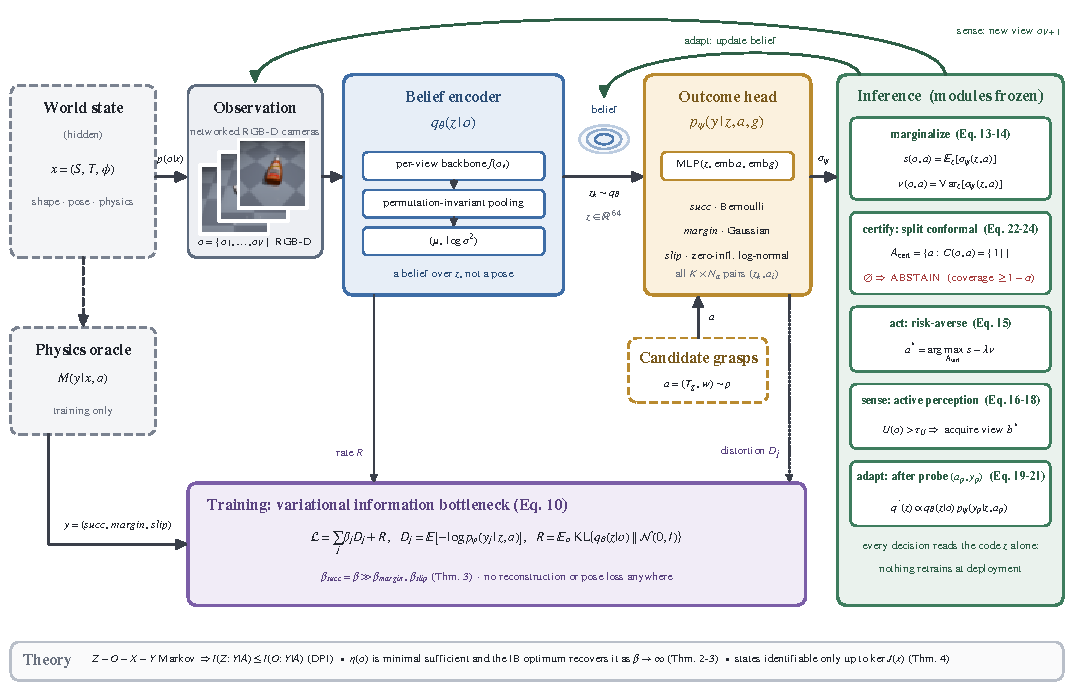
\includegraphics[width=0.92\textwidth]{figures/fig_framework.pdf}
\caption{Outcome-bottleneck interface. The sensor transmits the 128
parameters of $q_\theta(z\mid o)$. The decision node evaluates
$p_\psi(y\mid z,a)$ for candidate grasps and supports selection,
singleton-filtered abstention, active sensing, and probe assimilation.}
\label{fig:framework}
\end{figure*}

The sensor encodes each observation once, and the decision node queries many
grasps without retransmitting RGB-D data. Action conditioning preserves
within-scene grasp differences, while the two Gaussian parameter vectors
support repeated latent evaluation at a cost independent of candidate-set
size.

The state $x=(S,T,\phi)\in\mathcal X$ contains shape, pose
$T\in\mathrm{SE}(3)$, and $\phi=(\mu_f,m,c)$ for friction, mass, and center
of mass. Conditional on a fixed mesh, the identifiability calculation uses
\begin{equation}
x=\bigl(t,\,r,\,\log e,\,\log \mu_f,\,\log m,\,c\bigr)\in\R^{14},
\label{eq:state}
\end{equation}
where $t,r,e\in\R^3$ are translation, a fixed-branch local axis--angle
coordinate, and bounding-box half-extents. Mesh identity remains in $S$.
Observations are RGB-D images or view sets. A grasp is
$a=(t_a,r_a,w)\in\mathcal A=\mathrm{SE}(3)\times\R_{\ge0}$, using the same
rotation branch, and an optional $g\in\mathcal G$ specifies the gripper. The
outcome $y=(\suff,\mathrm{margin},\mathrm{slip})$ lies in
$\mathcal Y=\{0,1\}\times\R\times\R_{\ge0}$. A full-support target measure
$\rho$ defines relevance over actions, and
$M:\mathcal X\times\mathcal A\to\mathcal P(\mathcal Y)$ is the task kernel.
Under the target law,
\begin{equation}
\begin{aligned}
x&\sim p(x), & o&\sim p(o\mid x), & a&\sim\rho,\\
y&\sim M(\cdot\mid x,a), & z&\sim q_\theta(\cdot\mid o).&&
\end{aligned}
\label{eq:gen}
\end{equation}
where $q_\theta(z\mid o)$ and $p_\psi(y\mid z,a)$ are the encoder and outcome head.
Training draws from a boundary-focused proposal $\nu(\cdot\mid x)$ and uses
self-normalized weights $d\rho/d\nu$. The target is the posterior-predictive
outcome field
\begin{equation}
\begin{aligned}
\eta(o)&:=\bigl(a\mapsto p(y\mid o,a)\bigr),\\
p(y\mid o,a)&:=p(y\mid o,\mathrm{do}(A=a))\\
&=\int_{\mathcal{X}} M(y\mid x,a)\,p(x\mid o)\,dx.
\end{aligned}
\label{eq:eta}
\end{equation}

\begin{definition}[Manipulation sufficiency]
\label{def:sufficiency}
A representation kernel $q(z\mid o)$ is manipulation-sufficient iff
$Y\perp O\mid(Z,A)$ under~\eqref{eq:gen}, equivalently
$I(Z;Y\mid A)=I(O;Y\mid A)$. For $Z=t(O)$ this reduces to
$p(y\mid o,a)=p(y\mid t(o),a)$ for $\rho$-a.e.\ $a$.
\end{definition}

We assume measurable densities, a queryable training kernel, realizable
$p_\psi$, and full support of $\rho$. The identifiability result additionally
assumes a smooth state space and locally constant Jacobian rank; conformal
coverage assumes exchangeable independent scenes with outcome-independent
action randomization. Active sensing uses a predictive or learned gain model,
and probes have known transitions.

\section{The Manipulation-Sufficiency Objective}
\label{sec:objective}

Minimizing $I(Z;O)-\beta I(Z;Y\mid A)$ and applying standard variational
bounds~\cite{alemi2017} gives
\begin{equation}
\mathcal{L}(\theta,\psi)\;=\;\sum_{j\in\{\suff,\mathrm{m},\mathrm{s}\}}
\beta_j\, D_j(\theta,\psi)\;+\;R(\theta),
\label{eq:loss}
\end{equation}
where $D_j$ is coordinate-wise outcome log-loss and
$R=\E_o\KL(q_\theta(z\mid o)\|p_0(z))$. Outcome-specific $\beta_j$ prevents
likelihood scale from setting task priority; unless noted,
$\beta_{\mathrm m}=\beta_{\mathrm s}=10^{-2}$.

The encoder is a diagonal Gaussian
$q_\theta(z\mid o)=\mathcal{N}(\mu_\theta(o),\mathrm{diag}\,\sigma^2_\theta(o))$
with $p_0=\mathcal{N}(0,I_d)$ and reparameterized samples~\cite{kingma2014},
giving
\begin{equation}
\KL\bigl(q_\theta(z\mid o)\,\|\,p_0\bigr)=\tfrac12\sum_{j=1}^{d}
\bigl(\sigma_j^2+\mu_j^2-1-\log\sigma_j^2\bigr).
\label{eq:klclosed}
\end{equation}
The head factorizes as
\begin{equation}
\begin{split}
p_\psi(y\mid z,a)={}&\mathrm{Bern}\bigl(\suff;\varsigma(f_\psi(z,a))\bigr)\\
&\cdot\mathcal{N}\bigl(\mathrm{margin};m_\psi,\tau_\psi^2\bigr)\\
&\cdot\mathrm{ZILN}\bigl(\mathrm{slip};\pi_\psi,\nu_\psi,
\varrho_\psi^2\bigr),
\end{split}
\label{eq:headfactor}
\end{equation}
where $\varsigma$ is logistic and ZILN is zero-inflated log-normal.

With $K$ encoder samples, posterior-average and marginal-mixture estimators are
\begin{align}
\hat D^{\mathrm{post}}&=\frac1K\sum_{k=1}^{K}-\log p_\psi(y\mid z_k,a),
\label{eq:estimators}\\
\hat D^{\mathrm{marg}}&=-\log\frac1K\sum_{k=1}^{K} p_\psi(y\mid z_k,a).
\nonumber
\end{align}

Jensen gives $\E\hat D^{\mathrm{post}}\ge\E\hat D^{\mathrm{marg}}$. We use
$\hat D^{\mathrm{marg}}$, which consistently estimates the mixture log-loss
consumed at inference, with $K=8$ and a 15-epoch rate anneal. The resulting
finite model is a rate-regularized mixture predictor, not a proven minimal
sufficient statistic.

\begin{theorem}[Ideal minimal sufficiency]
\label{thm:ib}
The field $\eta(o)$ in~\eqref{eq:eta} is minimal sufficient. If the constraint
$I(Z;Y\mid A)=I(O;Y\mid A)$ is attainable, a deterministic minimizer of
$I(Z;O)$ subject to it induces the $\eta$-partition up to null sets.
\end{theorem}
\begin{proof}
Construction makes $\eta$ sufficient. For any sufficient $t$,
$p(y\mid o,a)=p(y\mid t(o),a)$, hence $\eta$ is a measurable function of $t$
and is minimal~\cite{lehmann1998}. The information equality is precisely
sufficiency, so minimum rate selects the coarsest deterministic partition.
\end{proof}

\section{Identifiability: What Outcomes Cannot Tell}
\label{sec:identifiability}

Rotations use the fixed logarithm chart $\|r\|<\pi$, and the coordinates in
Equation~\eqref{eq:state} use the Euclidean metric. For a finite probe set
${\{a_j\}}_{j=1}^{N}$, define
$\Phi_N(x)={\bigl(\vartheta_j(x)\bigr)}_{j\le N}\in\R^{Np}$, each $M(\cdot\mid x,a_j)$
represented by a finite sufficient parameter vector $\vartheta_j(x)\in\R^p$
(success logit, margin and slip moments), with differential
\begin{equation}
J_N(x):T_x\mathcal{X}\to\R^{Np},\qquad
J_N(x)\,\delta={\bigl(D_x\vartheta_j(x)[\delta]\bigr)}_{j\le N}.
\label{eq:jacobian}
\end{equation}
$\Phi_N$ diagnoses only the selected finite probe family; no dense-probe
derivative limit is assumed.

\begin{theorem}[Local identifiability, finite-probe form]
\label{thm:identifiability}
Under the smoothness and constant-rank assumptions, the level set
$\Phi_N^{-1}(\Phi_N(x))$ is, near $x$, a
smooth submanifold with
\begin{equation}
\begin{aligned}
T_x\,\Phi_N^{-1}(\Phi_N(x))&=\ker J_N(x),\\
\dim&=\dX-\mathrm{rank}\,J_N(x).
\end{aligned}
\label{eq:kernel}
\end{equation}
The locally identifiable component of any readout differential $dg$ is its
projection onto ${\bigl(\ker J_N(x)\bigr)}^{\perp}$.
\end{theorem}
\begin{proof}
The constant-rank theorem~\cite{lee2012} gives the submanifold and tangent
space $\ker D_x\Phi_N(x)=\ker J_N(x)$.
\end{proof}

Rank deficiency identifies continuous local ambiguity; full rank gives a
zero-dimensional local level set but may retain isolated global ambiguities.
Full-state metrics can therefore penalize probe-null directions invisible to
the outcome family.

\section{Inference: Decide, Filter, Sense, Adapt}
\label{sec:inference}

Deployment uses the trained encoder and outcome head; only the optional
view-acquisition regressor is additional.

\subsection{Decision Rule}
\label{sec:decision}
Given $o$, draw $K$ encoder samples $z_1,\dots,z_K\sim q_\theta(\cdot\mid o)$
and define, for each candidate action $a$,
\begin{align}
s(o,a)&=\E_{z\sim q}\bigl[\varsigma(f_\psi(z,a))\bigr]\nonumber\\
&\approx\frac1K\sum_{k}\varsigma(f_\psi(z_k,a)),
\label{eq:smean}\\
v(o,a)&=\mathrm{Var}_{z\sim q}\bigl[\varsigma(f_\psi(z,a))\bigr]\nonumber\\
&\approx\frac1K\sum_{k}{\bigl(\varsigma(f_\psi(z_k,a))-s\bigr)}^2.
\label{eq:svar}
\end{align}
$s$ is the mixture success probability and $v$ its induced latent-sampling
variance; neither is treated as a calibrated Bayesian posterior. Selection
is risk-averse over $\mathcal{A}_{\mathrm{cand}}\sim\rho$:
\begin{equation}
a^\ast(o)=\arg\max_{a\in\Afilt(o)}\;
\bigl[s(o,a)-\lambda\,v(o,a)\bigr],\qquad\lambda\ge0,
\label{eq:selection}
\end{equation}
The system filters first and selects second; pairwise coverage does not
automatically cover the selected extreme.

\subsection{Pairwise Conformal Filtering and Abstention}
\label{sec:conformal}
For the distribution-free construction, the exchangeability unit is a scene.
From each of $n$ independent calibration scenes, select one action index by a
prespecified randomization independent of its outcomes, giving a held-out fold
${\bigl\{(o_i,a_i,\suff_i)\bigr\}}_{i=1}^{n}$ disjoint from training. Compute
nonconformity scores
\begin{equation}
E_i=\begin{cases}1-s(o_i,a_i), & \suff_i=1,\\[2pt]
s(o_i,a_i), & \suff_i=0,\end{cases}
\label{eq:scores}
\end{equation}
and let $\hat q$ be the $\lceil(n{+}1)(1{-}\alpha)\rceil$-th smallest score,
taken as an order statistic. The prediction and retained-action sets are
\begin{align}
C(o,a)&=\bigl\{\ell\in\{0,1\}:\;\mathrm{score}_\ell(o,a)\le\hat q\bigr\},
\label{eq:predset}\\
\Afilt(o)&=\bigl\{a\in\mathcal{A}_{\mathrm{cand}}:\;C(o,a)=\{1\}\bigr\},
\label{eq:certset}
\end{align}
with $\mathrm{score}_1=1-s$ and $\mathrm{score}_0=s$. If
$\Afilt(o)=\varnothing$ the system abstains. Requiring the singleton $\{1\}$
rejects ambiguous $\{0,1\}$ sets that a one-sided threshold would admit.

\begin{theorem}[Marginal pairwise coverage]
\label{thm:coverage}
Let each calibration pair be obtained from an independent scene by the same
outcome-independent action randomization, and let the test pair be generated
likewise from a fresh scene. Then
$\Prob\bigl(\suff\in C(o,a)\bigr)\ge1-\alpha$.
\end{theorem}
\begin{proof}
Split-conformal validity~\cite{vovk2005}: the score is computed with a model
fit disjoint from calibration, so calibration and test scores are exchangeable
and the rank argument gives the bound.
\end{proof}

The theorem covers a randomized pair, not the selected maximizer. The scanned
diagnostic pools eight actions per scene and is therefore descriptive.

Under nonexchangeable deployment drift, the following adaptive-level
recursion is evaluated, motivated by adaptive conformal
inference~\cite{gibbs2021adaptive}:
\begin{equation}
\alpha_{t+1}=\alpha_t+\gamma\,(\alpha-\mathrm{err}_t),
\label{eq:aci}
\end{equation}
where $\alpha$ is fixed, $\mathrm{err}_t$ indicates miscoverage, and $\gamma$
is a step size. The unprojected bounded recursion has time-average error
converging to $\alpha$~\cite{gibbs2021adaptive}; Table~\ref{tab:drift} reports
only a full-feedback stress test, because abstentions do not provide labels.

\subsection{One Outcome Model for Sensing and Adaptation}
\label{sec:active}
Define the outcome-space ambiguity
\begin{equation}
U(o)=\E_{a\sim\rho}\bigl[v(o,a)\bigr]\;\approx\;
\frac{1}{|\mathcal{A}_{\mathrm{cand}}|}\sum_{a}v(o,a),
\label{eq:ambiguity}
\end{equation}
a per-scene scalar, never reduced over a batch, because sensing is a
per-scene decision.

\emph{Active viewpoint selection.}
For a sensing action $b\in\mathcal{B}$ with next-observation predictive
$\tilde p(o_b\mid o,b)$, the one-step value of information is
\begin{equation}
\mathrm{IG}(b)=U(o)-\E_{o_b\sim\tilde p}\bigl[U(o\cup o_b)\bigr],
\qquad b^\ast=\arg\max_b \mathrm{IG}(b),
\label{eq:ig}
\end{equation}
where fused views are re-encoded jointly. Simulation supplies exact rendered
look-ahead targets for an amortized gain regressor; deployment senses only when
\begin{equation}
U(o)>\tau_U
\label{eq:trigger}
\end{equation}
and budget remains. A permutation-invariant encoder fuses the view set.

\emph{Test-time adaptation.}
Executing probe $a_p$ and observing $y_p$ gives the latent target
$q'(z)\propto q_\theta(z\mid o)p_\psi(y_p\mid z,a_p)$, approximated with
$q'=\mathcal{N}(\mu',\mathrm{diag}\,\sigma'^2)$ initialized at
$q_\theta(\cdot\mid o)$,
\begin{equation}
\min_{\mu',\sigma'}\;\E_{z\sim q'}\bigl[-\log p_\psi(y_p\mid z,a_p)\bigr]
+\KL\bigl(q'\,\|\,q_\theta(\cdot\mid o)\bigr),
\label{eq:tta}
\end{equation}
using a few projected gradient steps and $\|\mu'-\mu\|\le\delta$. With unit
KL weight this is the Gaussian-family projection of the auxiliary Bayesian
update; the encoder is not claimed to be a physical-state posterior. Probe
adaptation is evaluated only on the synthetic oracle.

\subsection{Implementation and Complexity}
\label{sec:algorithms}
Training renders a scene, samples importance-weighted actions, evaluates all
$K\times N_a$ latent--action pairs, and updates~\eqref{eq:loss} with a
15-epoch rate anneal. A disjoint fold determines $\hat q$. At deployment the
sensor encodes once; the decision node evaluates~\eqref{eq:smean}--\eqref{eq:svar},
optionally acquires a view when~\eqref{eq:trigger} holds, applies the singleton
test~\eqref{eq:certset}, selects~\eqref{eq:selection}, and optionally
updates~\eqref{eq:tta}. The encoder costs $O(F)$ and the head $O(KN_a h)$.
Table~\ref{tab:interface} reports a 16.2\,ms two-core cycle and 512\,B payload.

\begin{table}[t]
\centering
\caption{Measured interface budget (Ours; primary $\alpha{=}0.1$
checkpoint, fp32, two x86-64 CPU cores, median of 60 runs). No GPU or
accelerator is used.}
\label{tab:interface}
\begin{tabular}{lr}
\toprule
Quantity & Value \\
\midrule
Encoder parameters & 11.41\,M \\
Head parameters & 0.251\,M \\
Encoder payload $(\mu,\log\sigma^2)$, fp32 & 512\,B \\
Single RGB-D frame, fp32 & 147.5\,kB \\
Eight-view set, fp32 & 1.18\,MB \\
Encoder forward, 1 / 2 threads & 25.6 / 14.9\,ms \\
Head, $K{=}32\times N_a{=}8$, 1 / 2 threads & 2.1 / 1.3\,ms \\
Perceive-and-score cycle, 1 / 2 threads & 27.7 / 16.2\,ms \\
\bottomrule
\end{tabular}
\end{table}
Optional sensing adds one amortized forward pass per candidate viewpoint;
optional adaptation adds $O(k)$ head evaluations for $k$ gradient steps,
with the encoder fixed. Neither path reconstructs geometry or performs a
dynamics rollout at deployment. Table~\ref{tab:interface} is a single-system
measurement; matched-rate JPEG, neural-codec, VL-VFE, and quantized-interface
accuracy rows remain unmeasured.

\section{Experimental Setup and Evaluation Protocol}
\label{sec:setup}
\subsection{Physics Stack and Corpus}
The analytic tier evaluates differentiable Ferrari--Canny quality on an
oriented bounding box using eight-ray friction cones and a 140-direction
wrench-hull support approximation~\cite{ferrari1992planning}. The simulation
tier executes the same grasp in MuJoCo on the true convex decomposition with
sampled mass, friction, and center of mass~\cite{todorov2012}. Jaws close for
300 steps at 2\,ms, settle for 100, lift 0.12\,m at 0.15\,m/s, and hold for
400; success requires 0.05\,m clearance. Training uses
\begin{equation}
\begin{aligned}
M_{\mathrm{train}}(dy\mid x,a)={}&
M_{\mathrm{sim}}(d\suff,d\mathrm{slip}|x,a)\\
&\cdot\delta_{m_{\mathrm{box}}(x,a)}(d\mathrm{margin}).
\end{aligned}
\label{eq:hybridkernel}
\end{equation}
so success and slip come from simulation and the downweighted margin is
analytic. Across 320 matched grasps, analytic and simulated success rates are
0.68 and 0.25, agreement is 0.42, the analytic false-positive rate is 0.74,
and analytic versus dynamic slip has $r=-0.02$. Conclusions therefore concern
this reconstruction, metric, simulator, and candidate set.

Both tiers receive the same scene and grasp. The analytic tier supplies the
auxiliary margin and comparison score; simulation supplies lift and slip.
Consequently, the reconstruction model does not define its own evaluation
target, and disagreement isolates the effect of replacing the true contact
geometry with the bounding-box approximation.

The corpus contains 13 LIBERO grocery meshes, six box-hulled and seven
curved~\cite{liu2023libero}. Settled scenes randomize yaw, position,
$\log\mu_f\sim\mathcal N(\log0.8,0.3^2)$,
$\log m\sim\mathcal N(\log0.25,0.5^2)$, and center of mass. Each has eight
candidate grasps and eight $96\times96$ RGB-D views. Train/validation/
calibration/test folds contain 8{,}000/1{,}000/2{,}000/2{,}000 scenes; 11{,}979
of 16{,}000 test pairs are executable. Base success is 0.597 and object rates
span 0.043 to 0.999.

Training is scene-based: the encoder runs once and the head evaluates all
$K\times N_a$ latent--action pairs. Actions follow the boundary-focused
proposal $\nu$, with self-normalized $d\rho/d\nu$ weights preserving the
target measure $\rho$.

\begin{figure*}[t]
\centering
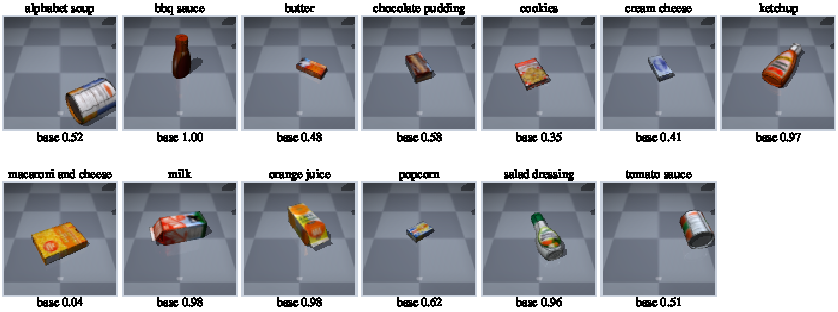
\includegraphics[width=\textwidth]{figures/fig_objects.pdf}
\caption{The thirteen HOPE grocery meshes, one test scene each, with the per-object base
success rate over executable grasps. The range from 0.04 to 1.00 is why ablations are
refereed on within-scene AUC: a pooled score can be reached by learning object identity
alone.}
\label{fig:objects}
\end{figure*}

\begin{table}[t]
\centering\small
\caption{Grasp corpus. 13 HOPE grocery meshes on a table, 8 RGB-D views per
scene at $96{\times}96$, 8 sampled parallel-jaw grasps per scene, outcome
labels from MuJoCo {\tt 3.10.0} rollouts. A grasp is inexecutable when the open jaws already
intersect the scene; success rate is reported over executable grasps only. Splits are drawn with
disjoint seeds and the calibration split is held disjoint from training, as the conformal
guarantee requires.}
\label{tab:dataset}
\begin{tabular}{lrrrrrr}
\toprule
Split & Seed & Scenes & Grasps & Executable & Exec.\ (\%) & Success (\%) \\
\midrule
Train & 1 & 8,000 & 64,000 & 48,268 & 75.4 & 61.7 \\
Val & 2 & 1,000 & 8,000 & 6,066 & 75.8 & 62.2 \\
Calibration & 3 & 2,000 & 16,000 & 11,935 & 74.6 & 61.4 \\
Test & 4 & 2,000 & 16,000 & 11,979 & 74.9 & 59.7 \\
\midrule
Total & -- & 13,000 & 104,000 & 78,248 & & \\
\bottomrule
\end{tabular}
\end{table}

\begin{figure}[t]
\centering
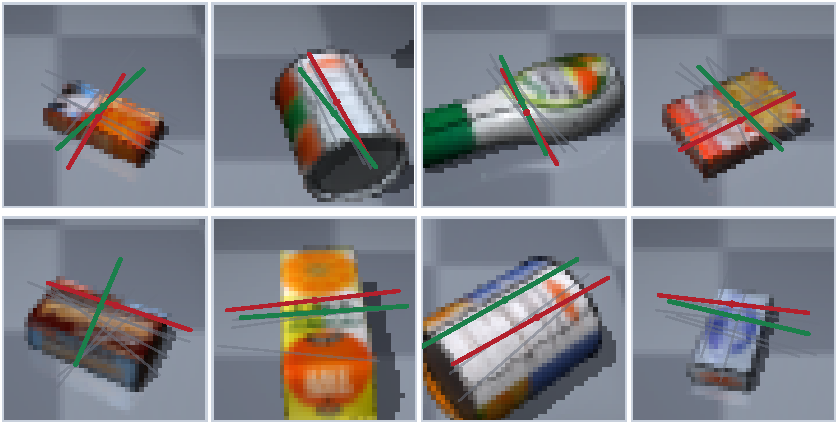
\includegraphics[width=\columnwidth]{figures/fig_qualitative.pdf}
\caption{Eight test scenes, one per object. Grey segments are the candidate jaw axes,
green is the grasp our score ranks first and the simulator lifts, red is the grasp the
analytic proxy ranks first and the simulator drops. Panels are cases where the two
selectors disagree; the population comparison is Table~\ref{tab:baselines}.}
\label{fig:qualitative}
\end{figure}

\subsection{Training, Baselines, and Metrics}
The encoder is a four-channel ResNet-18~\cite{he2016} producing
$(\mu,\log\sigma^2)\in\R^{128}$; mean pooling fuses views. A 256-unit action
embedding is feature-wise modulated by $z$, and the head emits the parameters
in~\eqref{eq:headfactor}. AdamW uses learning rate $5\times10^{-4}$, weight decay
$10^{-4}$, batch size 128, 60 epochs, $K=8$, a 15-epoch rate anneal, and a
10-epoch deterministic warmup. Unless noted,
$(\beta_{\suff},\beta_{\mathrm m},\beta_{\mathrm s})=(300,10^{-2},10^{-2})$;
filtering uses $\beta_{\suff}=30$ and the frontier sweeps
$\{1,3,10,30,100\}$.

At evaluation, each observation is encoded once and the decision node draws
$K=32$ latent samples to estimate the mean and variance in
Equations~\eqref{eq:smean}--\eqref{eq:svar} for all eight candidate actions.
The same candidate set is supplied to every ranking method, so differences in
top-1 and selective success arise from scoring rather than proposal quality.
Active-view experiments use separate Monte Carlo draws for viewpoint choice
and final scoring to avoid evaluating a selected view on the noise realization
that selected it.

The four folds have distinct roles. The training fold updates
$(\theta,\psi)$, the validation fold selects checkpoints and operating
settings, the calibration fold estimates conformal quantiles, and the test
fold supplies every reported comparison. Keeping quantile estimation separate
from checkpoint selection prevents test outcomes from influencing either the
predictor or its filtering threshold. For leave-one-object-out evaluation,
this sequence is repeated after removing the held-out object from all three
development folds.

A 6-D synthetic oracle with rank-three $J_N$ provides known invariant
subspaces and 64{,}000 independent test points.

Evaluation preserves the unit associated with each claim. Action-level AUC
uses the 11{,}979 executable test pairs. Top-1 and selective success operate
on 1{,}997 scenes after ranking the available candidates. The independent
synthetic points support the finite-sample conformal test, whereas the
16{,}000 scanned action records are retained only for the explicitly
clustered all-pair diagnostic. Identifiability compares local subspaces rather
than prediction scores, and the interface benchmark times one encoder pass
plus the complete $K{=}32$, $N_a{=}8$ head evaluation. These denominators are
reported separately because action prediction, scene selection, coverage,
and local geometry agreement have different sampling units.

Metrics are pooled and within-scene AUC, top-1 and selective success,
coverage, singleton precision, abstention, retained-action fraction, KL rate,
and payload size. Within-scene AUC averages scenes containing both labels and
prevents object base rate from substituting for grasp ranking. Baselines are
random or majority prediction, bounding-box Ferrari--Canny quality, and an
MLP on the privileged 14-D state. The conformal theorem uses one prespecified
action per independent scene; scanned all-pair values are clustered empirical
diagnostics. Three full-model seeds give within-scene AUC
$0.635\pm0.011$, pooled AUC $0.875\pm0.002$, top-1 $0.692\pm0.008$, and
selective success $0.976\pm0.008$ (mean $\pm$ sd); ablations use one seed.

\emph{Comparator scope.} All reported numbers are measured on this corpus.
Released grasping checkpoints require incompatible crops, point clouds, TSDFs,
cameras, or grippers, and were not evaluated zero-shot. The available
artifacts also do not contain measurements for Ferrari--Canny on true contact
geometry, combined analytic metrics, a matched-capacity deterministic BCE
scorer, retrained Dex-Net/6-DOF evaluators, rate-matched reconstruction or
VL-VFE, an oracle ceiling, or matched-abstention softmax, MC-dropout, and
ensemble confidence~\cite{geifman2017selective,gal2016dropout,%
lakshminarayanan2017}. Consequently, E1 and E2 are controlled diagnostics
against the measured OBB proxy, not state-of-the-art baseline claims; these
comparisons are required before a definitive superiority claim.

Pooled AUC ranks all executable records and can exploit object base rates;
within-scene AUC averages only mixed-label scenes and measures grasp ordering
for a fixed observation. Top-1 success evaluates the highest-ranked candidate,
whereas selective success also thresholds scene confidence. Coverage concerns
prediction-set inclusion, while singleton precision is conditional on
retention. Each scene is treated as a cluster because its eight actions share
observations and physical parameters. All ranking methods use the same
candidates. The privileged 14-D baseline supplies pose and physical variables
but is not an upper bound because it omits mesh identity and surface geometry.

\section{Results}
\label{sec:results}

\subsection{E1: Controlled OBB Analytic Diagnostic}
\label{sec:e1}
This experiment asks whether Ferrari--Canny computed on the OBB reconstruction
ranks realized lifts. It does not separate reconstruction error from metric
error; that requires the unmeasured true-geometry and combined-metric rows.

\begin{table}[t]
\centering
\caption{Measured predictive validity on 11{,}979 executable grasps; base
success is 0.597. Ferrari--Canny uses the OBB reconstruction. The privileged
MLP omits mesh identity and is not an upper bound.}
\label{tab:proxy}
\small
\begin{tabular}{lccc}
\toprule
Predictor & Pooled & Within-scene & Best acc.\\
\midrule
Chance / majority & 0.500 & 0.500 & 0.597 \\
Ferrari--Canny (recon.) & 0.542 & 0.548 & 0.612 \\
\textbf{Ours} & \textbf{0.876} & \textbf{0.639} & \textbf{0.784} \\
\midrule
\emph{Privileged state} & -- & \emph{0.685} & -- \\
\bottomrule
\end{tabular}
\end{table}

Table~\ref{tab:proxy} shows 0.542/0.548 pooled/within-scene AUC for the
analytic proxy and 0.876/0.639 for ours; the privileged-state baseline reaches
0.685 within-scene. The proxy's best accuracy, 0.612, barely exceeds the
0.597 majority floor.

Stratification localizes the proxy failure: AUC is 0.574
on exact box hulls but 0.473 on curved objects, while ours reaches 0.797 and
0.891. This correlation with reconstruction mismatch is suggestive, but only
a true-geometry Ferrari--Canny row can isolate geometry error from metric
error~\cite{rubert2017relevance,lu2022hybrid}.

\subsection{E2: Selective Execution}
\label{sec:selective}
For each method, the scene confidence is the score of its own selected
top-ranked action: $s-\lambda v$ for ours and the Ferrari--Canny value for the
analytic baseline. The 25\% operating point retains the top quartile of scenes
under that method-specific score.

\begin{table}[t]
\centering
\caption{Measured selective execution over 1{,}997 scenes. Each method uses
its own confidence score; this is not a matched-abstention comparison against
learned uncertainty baselines.}
\label{tab:selective}
\begin{tabular}{lcc}
\toprule
Act rate & Ferrari--Canny & \textbf{Ours} \\
\midrule
0.25 (selective) & 0.503 & \textbf{0.984} \\
1.00 (always act) & 0.665 & \textbf{0.692} \\
\midrule
Random grasp & \multicolumn{2}{c}{0.623} \\
\bottomrule
\end{tabular}
\end{table}

Table~\ref{tab:selective} reports the operating points. Stronger selection
improves our executed-grasp success to 0.984 at 25\% commitment, whereas the
proxy falls to 0.503, below its 0.665 always-act rate. The opposite trends
show that the learned score orders both actions within a scene and confidence
across scenes better than this OBB proxy. They do not establish an advantage
over temperature-scaled thresholds, MC dropout, or deep ensembles at matched
abstention.

\subsection{E3: Pairwise Filtering and Coverage Diagnostics}
\label{sec:coverage-results}
The synthetic oracle tests Theorem~\ref{thm:coverage} on independent points;
the scanned corpus pools eight actions per scene and is descriptive.

\begin{table}[t]
\centering
\caption{Empirical singleton filtering on the scanned-object corpus
($\beta_{\suff}=30$; 16{,}000 action records over $\approx$2{,}000 scenes).
Because calibration pooled eight correlated actions per scene, these values
are descriptive and Theorem~\ref{thm:coverage} does not apply. Singleton
precision is a distinct selection-conditional estimand.}
\label{tab:coverage}
\begin{tabular}{lccc}
\toprule
 & $\alpha=0.05$ & $\alpha=0.10$ & $\alpha=0.20$ \\
\midrule
Target coverage $1-\alpha$ & 0.950 & 0.900 & 0.800 \\
Pairwise coverage (\textbf{Ours}) & \textbf{0.946} & \textbf{0.897} &
\textbf{0.800} \\
Singleton precision & 0.792 & 0.744 & 0.673 \\
Abstention rate & 0.823 & 0.743 & 0.598 \\
Retained action fraction & 0.169 & 0.235 & 0.373 \\
\bottomrule
\end{tabular}

\end{table}

Table~\ref{tab:coverage} gives scanned all-pair coverage
0.946/0.897/0.800 against 0.950/0.900/0.800. The independent synthetic oracle gives
0.979/0.949/0.901/0.802/0.700 against targets
0.98/0.95/0.90/0.80/0.70. At $\alpha=0.1$, the scanned filter retains 23.5\% of
actions; increasing $\beta_{\suff}$ to 100 reduces abstention to 0.367.

\begin{figure*}[!t]
\centering
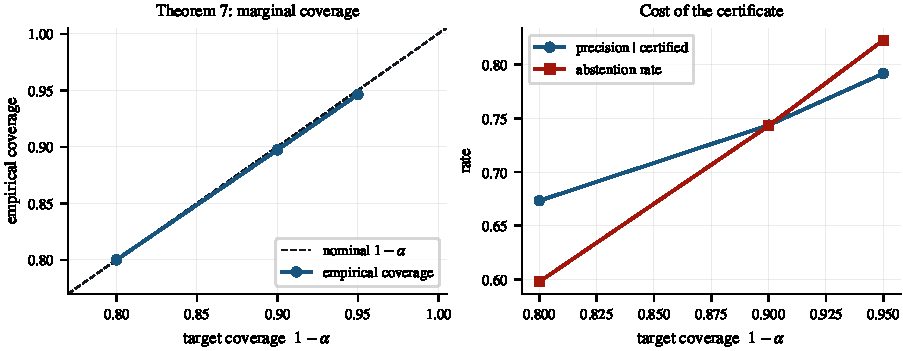
\includegraphics[width=0.82\textwidth]{figures/fig_coverage.pdf}
\caption{Independent synthetic-oracle coverage tracks the tested targets;
the right panel relates empirical coverage to the KL rate surrogate.}
\label{fig:coverage}
\end{figure*}

Under object-sorted full-feedback drift, the anchored update raises the worst
500-decision window from 0.702 to 0.744 and the worst object from 0.720 to
0.834, while reducing per-object dispersion from 0.111 to 0.035
(Table~\ref{tab:drift}).

\begin{table}[t]
\centering
\caption{Empirical coverage under an object-sorted stream (Ours; 16{,}000
decisions sorted by object, target 0.90), a full-feedback stress test:
every decision supplies a label, unlike the selective feedback of a deployed
policy that abstains. The fixed column uses the calibration-fold quantile; the
ACI column uses~\eqref{eq:aci} with $\gamma=0.01$. Marginal coverage is
order-invariant; local coverage is not.}
\label{tab:drift}
\begin{tabular}{lcc}
\toprule
 & Fixed $\hat q$ & ACI (anchored) \\
\midrule
Marginal coverage & 0.899 & \textbf{0.900} \\
Worst 500-decision window & 0.702 & \textbf{0.744} \\
Worst object segment & 0.720 & \textbf{0.834} \\
Per-object dispersion (std) & 0.111 & \textbf{0.035} \\
\bottomrule
\end{tabular}
\end{table}

\subsection{E4: Identifiability, Predicted vs.\ Measured}
\label{sec:ident-results}
The synthetic oracle differentiates its true kernel; the scanned experiment
compares the analytic bounding-box Jacobian with measured simulator
invariances.

\begin{table}[t]
\centering
\caption{Finite-probe identifiability. The angle compares the analytic
$\ker J_N(x)$ with the simulator's measured invariant subspace; a dash marks
a full-rank Jacobian.}
\label{tab:ident}
\footnotesize
\begin{tabular}{lrrr}
\toprule
Object & Rank & Nullity & Angle [$^\circ$] \\
\midrule
alphabet soup & 12 & 2 & 0.05 \\
BBQ sauce & 14 & 0 & -- \\
butter & 14 & 0 & -- \\
chocolate pudding & 14 & 0 & -- \\
cookies & 14 & 0 & -- \\
cream cheese & 14 & 0 & -- \\
ketchup & 13 & 1 & 0.05 \\
macaroni and cheese & 13 & 1 & 0.04 \\
milk & 11 & 3 & 0.21 \\
orange juice & 12 & 2 & 0.55 \\
popcorn & 14 & 0 & -- \\
salad dressing & 12 & 2 & 0.06 \\
tomato sauce & 12 & 2 & 0.06 \\
\bottomrule
\end{tabular}
\end{table}

The synthetic oracle verifies the finite-probe calculation: the mean and
maximum principal angles are $0.013^{\circ}$ and
$0.056^{\circ}$ over 50 states, with exact rank and nullity. On the scanned
corpus, Table~\ref{tab:ident} shows seven rank-deficient objects with
analytic-to-simulator angles below $0.56^{\circ}$; the other six have
full-rank $J_N$ and locally zero-dimensional analytic level sets. This
agreement supports the surrogate as a local diagnostic, not as the Jacobian
of the true physics.

\begin{figure}[!t]
\centering
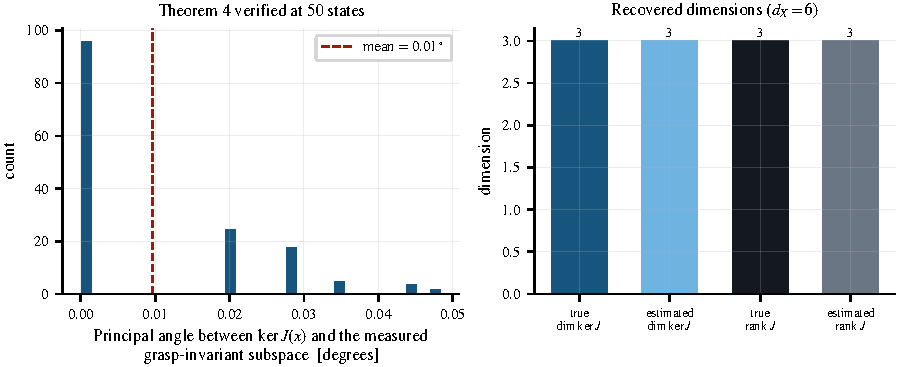
\includegraphics[width=0.95\columnwidth]{figures/fig_identifiability.pdf}
\caption{Synthetic-oracle verification recovers rank and nullity exactly;
predicted and measured invariant subspaces agree within $0.056^{\circ}$.}
\label{fig:ident}
\end{figure}

\subsection{E5: The Rate-Distortion Frontier}
\label{sec:frontier}
Increasing $\beta_{\suff}$ emphasizes success log-loss at the cost of a
larger KL rate surrogate.

\begin{table}[!t]
\centering
\caption{Rate-distortion frontier (16{,}000 test pairs per row). Larger
$\beta$ emphasizes success prediction; coverage is the clustered all-pair
diagnostic.}
\label{tab:frontier}
\begin{tabular}{rccccc}
\toprule
$\beta$ & $R$ [nats] & $D_{\suff}$ & $\sum_j D_j$ & Coverage &
Abstention \\
\midrule
1 & 0.004 & 0.656 & 0.725 & 0.896 & 0.643 \\
3 & 0.088 & 0.622 & 0.767 & 0.892 & 0.674 \\
10 & 0.280 & 0.598 & 0.870 & 0.904 & 0.736 \\
30 & 0.534 & 0.582 & 0.993 & 0.897 & 0.743 \\
100 & 3.286 & \textbf{0.412} & 0.956 & 0.905 & \textbf{0.367} \\
\bottomrule
\end{tabular}
\end{table}

Table~\ref{tab:frontier} shows the expected rate-distortion trend: as $R$
rises from 0.004 to 3.29 nats,
$D_{\suff}$ falls from 0.656 to 0.412, while coverage remains 0.892--0.905.
From $\beta=30$ to 100, abstention falls from 0.743 to 0.367. The measured
payload is 512\,B in fp32, $288\times$ smaller than one frame; $R$ remains a
KL surrogate rather than an implemented code length~\cite{havasi2019}.

\subsection{E6: Active Perception with Independent Scoring}
\label{sec:active-results}
A random second view reduces $U(o)$ by 13.8\%; selecting with~\eqref{eq:ig}
and scoring on independent Monte Carlo draws yields 16.7\%. The modest gain
indicates that much residual variation is not visually observable. This study
compares only with random view selection; closed-loop NBV and affordance-driven
methods were not reimplemented~\cite{breyer2022closed,zhang2023ace}.

\subsection{E7: Combined Deterministic and No-Rate Ablation}
\label{sec:baseline}
Setting $z=\mu$ and removing KL yields 0.527 within-scene AUC, 0.633 top-1
success, and 0.651 selective success, versus 0.639/0.692/0.984 for the full
model. Action response falls from 0.221 to 0.0008. This combined ablation
shows the configuration matters but neither separates sampling from KL nor
replaces the required matched-capacity deterministic BCE baseline.

\subsection{E8: Ablations}
\label{sec:ablations}
Action response is the standard deviation of $s(o,a)$ across a scene's
candidates; values near zero indicate collapsed grasp ranking.

\begin{table}[!t]
\centering
\caption{Ablations on the scanned-object corpus
($\beta_{\suff}=300$ except where the budget itself is ablated). Pooled AUC
can remain near 0.7 after within-scene ranking has collapsed.}
\label{tab:ablations}
\footnotesize
\setlength{\tabcolsep}{3pt}
\begin{tabular}{lccc}
\toprule
Variant & Within & Pooled & Resp. \\
\midrule
\textbf{Ours (full)} & \textbf{0.639} & 0.875 & 0.221 \\
Uniform outcome budget & 0.511 & 0.710 & 0.002 \\
Constant $z$ & 0.506 & 0.615 & 0.031 \\
$K{=}1$ sample & 0.602 & 0.844 & 0.174 \\
$d{=}16$ & 0.634 & 0.873 & 0.219 \\
$d{=}32$ & 0.587 & 0.846 & 0.185 \\
\bottomrule
\end{tabular}
\end{table}


Uniform outcome weighting and constant $z$ reduce within-scene AUC to
0.511 and 0.506, with action response 0.002 and 0.031
(Table~\ref{tab:ablations}). Using one sample gives 0.602 AUC\@; $d=16$ matches
the $d=64$ model at 0.634 versus 0.639. The $d=32$ result is single-seed and
falls within unresolved architecture variance. On the synthetic oracle,
singleton filtering raises success from 0.935 to 0.949 while abstaining on 9
of 400 episodes. Pooled and within-scene AUC differ because object base rates
vary widely, so pooled ranking can benefit from object recognition even when
grasp ordering within a scene is weak.

\subsection{E9: Generalization to Unseen Objects}
\label{sec:loo}
Thirteen models each hold out one object; filtering is calibrated on the
remaining twelve and evaluated on the unseen object. A second protocol withholds four
identities at once, which is the harder and more realistic shift.

Ranking does not transfer. Under the four-object shift the pooled AUC is 0.478 and the
within-scene AUC is 0.506, both at chance, against 0.886 and 0.690 on the objects seen in
training. What does transfer is the decision to stay silent: the certified fraction falls
from 0.46 to 0.037 while the certificates still issued remain 0.917 precise, and adaptive
calibration holds coverage at 0.877 against a 0.90 target. The interface withdraws instead
of misfiring, which is the property that matters when an unfamiliar object arrives, and we
do not claim that the scorer generalizes across object identity.

\begin{table}[t]
\centering
\caption{Leave-one-object-out transfer. Coverage uses an all-pair filter calibrated on the other twelve objects, with target 0.90.}
\label{tab:loo}
\scriptsize
\setlength{\tabcolsep}{2.5pt}
\begin{tabular}{lccccc}
\toprule
Held-out object & base & Within & Top-1 & Cov.\ fix & Cov.\ ACI \\
\midrule
\multicolumn{6}{l}{\emph{Moderate base rate ($0.3<\text{base}<0.7$):
within-scene AUC is meaningful}} \\
butter & 0.48 & 0.569 & 0.474 & 0.703 & 0.895 \\
cream cheese & 0.41 & 0.546 & 0.429 & 0.543 & 0.896 \\
tomato sauce & 0.51 & 0.511 & 0.473 & 0.785 & 0.896 \\
alphabet soup & 0.52 & 0.479 & 0.500 & 0.774 & 0.897 \\
choc.\ pudding & 0.58 & \textbf{0.695} & 0.778 & 0.845 & 0.898 \\
popcorn & 0.62 & 0.475 & 0.601 & 0.666 & 0.893 \\
cookies & 0.35 & \textbf{0.709} & 0.491 & 0.805 & 0.899 \\
\emph{subgroup mean} & & \emph{0.569} & \emph{0.535} & \emph{0.732} &
\emph{0.896} \\
\midrule
\multicolumn{6}{l}{\emph{Extreme base rate: within-scene AUC degenerate}} \\
macaroni & 0.04 & 0.497 & 0.028 & 0.625 & 0.780 \\
BBQ sauce & 1.00 & -- & 0.993 & 0.752 & 0.890 \\
salad dress. & 0.96 & 0.520 & 0.975 & 0.704 & 0.877 \\
ketchup & 0.97 & 0.546 & 0.975 & 0.533 & 0.853 \\
milk & 0.98 & 0.528 & 0.984 & 0.913 & 0.907 \\
orange juice & 0.98 & 0.422 & 0.974 & 0.820 & 0.898 \\
\emph{subgroup mean} & & \emph{0.503} & \emph{0.822} & \emph{0.724} &
\emph{0.868} \\
\midrule
\textbf{All objects} & & 0.541 & 0.667 & 0.728 & \textbf{0.883} \\
\bottomrule
\end{tabular}
\end{table}

For the seven moderate-base objects, within-scene AUC falls from 0.639 to
0.569; extreme-base objects contain too few mixed-label scenes for stable
ranking estimates (Table~\ref{tab:loo}). Mean all-pair coverage is 0.728 with
the fixed quantile and 0.883 after full-feedback adaptation, still below the
0.90 target. Transfer is therefore partial and object-dependent.


\subsection{E10: Learned Baselines and the Rate--Quality Frontier}
\label{sec:baselines}
Table~\ref{tab:baselines} scores every method on the same candidate grasps. Two learned
competitors matter. The first shares our backbone, latent width and action head with the
rate term removed, isolating the bottleneck: it reaches 0.653 within-scene AUC against our
0.640, so compression costs nothing in ranking but buys nothing either. The second is the
Dex-Net grasp-quality architecture retrained here on the same corpus, which reaches
$0.851 \pm 0.006$ within-scene AUC over three seeds and ranks grasps better than we do.
Its advantage is architectural: the depth patch is cropped and rotated by the candidate
pose, so the action enters through the receptive field rather than through a learned
conditioning path.

\begin{table}[t]
\centering\small
\setlength{\tabcolsep}{4pt}
\caption{Ranking quality and transport cost on the same candidate grasps. Payload is the
entropy-coded representation one scene must send to the decision node, in bytes; the
per-action column reflects that a grasp-aligned representation is formed after the action
is applied, so an edge deployment sends one per candidate. GQ-CNN ranks better when
bandwidth is unconstrained; MSP reaches its own operating point at two orders of magnitude
fewer bits, and is the stronger ranker at the tightest budget (Fig.~\ref{fig:frontier}).}
\label{tab:baselines}
\begin{tabular}{lccccc}
\toprule
& \multicolumn{3}{c}{Ranking} & \multicolumn{2}{c}{Payload (bytes)} \\
\cmidrule(lr){2-4}\cmidrule(lr){5-6}
Method & Pooled AUC & Within-scene & Top-1 & fp32 & 2-bit \\
\midrule
GQ-CNN architecture, retrained & 0.932 & 0.851 & 0.828 & 32768 & 251 \\
MSP (ours) & 0.875 & 0.640 & 0.698 & 256 & 10 \\
Direct success CNN, no bottleneck & 0.881 & 0.653 & 0.695 & -- & -- \\
Ferrari--Canny on reconstructed box & 0.542 & 0.548 & 0.665 & -- & -- \\
Random & 0.489 & 0.500 & 0.636 & -- & -- \\
\bottomrule
\end{tabular}
\end{table}

That advantage is paid for on the wire. A grasp-aligned representation exists only after a
grasp is chosen, so scoring $K$ candidates costs $K$ payloads, while a statistic formed
before the action is chosen costs one. Figure~\ref{fig:frontier} applies the same
quantizer to both and plots quality against measured entropy-coded bits. The curves cross
near 600 bits per scene. At the tightest budget our statistic reaches 0.591 within-scene
AUC from 48 bits where the baseline reaches 0.574 from 382, eight times fewer bits and a
better score; given two orders of magnitude more bandwidth the ordering reverses. Which
side of the crossing a deployment sits on is a link-budget question, not a modelling one.

\begin{figure}[t]
\centering
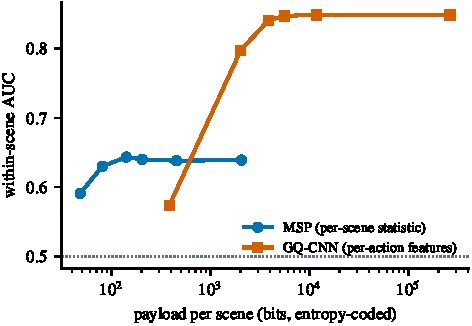
\includegraphics[width=0.95\columnwidth]{figures/fig_rate_frontier.pdf}
\caption{Rate--quality frontier under one quantizer. Our per-scene statistic saturates by
140 bits; the per-action baseline needs roughly 3{,}800 bits to saturate and 382 bits
before it beats chance by a useful margin.}
\label{fig:frontier}
\end{figure}

\subsection{E11: Transport Cost and Behaviour Under Loss}
\label{sec:transport}
Quantizing the belief to two bits per dimension and entropy coding the symbols gives 80.4
bits, ten bytes, per scene. Decisions recomputed from the dequantized belief are
indistinguishable from fp32: 0.636 against 0.638 within-scene AUC, 0.691 against 0.694
top-1 success, and 0.906 against 0.904 coverage. One bit per dimension is the cliff, at
0.584. The saving is 25-fold against the 2{,}048-bit fp32 representation, and at 1\,Mbit/s
the payload occupies the uplink for 0.33\,ms (Fig.~\ref{fig:ratesweep}).

Loss is the more informative axis. When a payload does not arrive the decision node holds
no belief and therefore certifies nothing, so the controller abstains. Sweeping loss from
0 to 20\% moves the fraction of scenes acted on from 0.628 to 0.507 while success given
action stays flat between 0.852 and 0.860. A degrading link costs throughput and does not
buy failed grasps (Fig.~\ref{fig:loss}), which is the behaviour a certificate is for.

\begin{figure}[t]
\centering
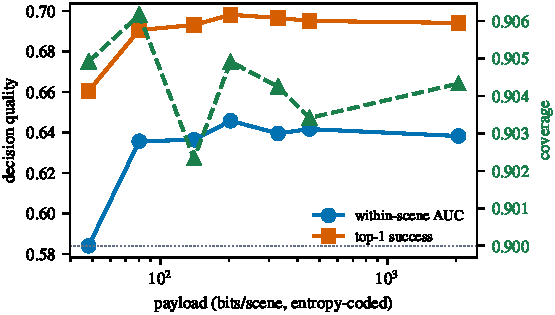
\includegraphics[width=0.95\columnwidth]{figures/fig_rate_sweep.pdf}
\caption{Decision quality and coverage against measured entropy-coded payload. Two bits
per dimension, ten bytes per scene, is indistinguishable from fp32; one bit is the cliff.}
\label{fig:ratesweep}
\end{figure}

\begin{figure}[t]
\centering
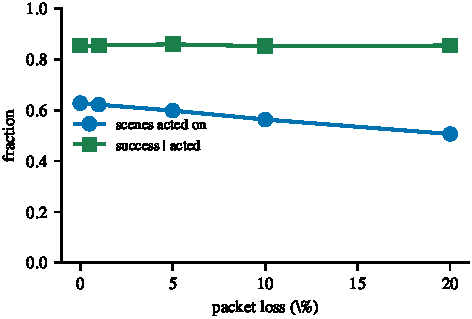
\includegraphics[width=0.95\columnwidth]{figures/fig_packet_loss.pdf}
\caption{A lossy uplink costs throughput, not reliability. As loss rises to 20\% the
fraction of scenes acted on falls from 0.628 to 0.507 while success given action stays
between 0.852 and 0.860.}
\label{fig:loss}
\end{figure}

\subsection{E12: Coverage for the Grasp That Is Executed}
\label{sec:selective}
The filter of Section~\ref{sec:conformal} is calibrated over observation--action pairs,
while the controller executes an $\arg\max$. Selection is data dependent, so the executed
pair is not exchangeable with the calibration pairs and the guarantee does not transfer to
it as stated. Calibrating instead on the selected action of each calibration scene applies
the same rule to both folds and restores exchangeability at the scene level.

Empirically the published filter is conservative rather than invalid on the executed
grasp, delivering 0.960 coverage at a 0.95 target, and the recalibrated filter is exact at
0.955 while raising the certified fraction from 0.372 to 0.510. At the 0.90 target the
three procedures give 0.904, 0.904 and 0.906 with certified fractions 0.456, 0.628 and
0.622. The scene-level statement is therefore both correct and less conservative, and we
adopt it throughout.

\begin{figure}[t]
\centering
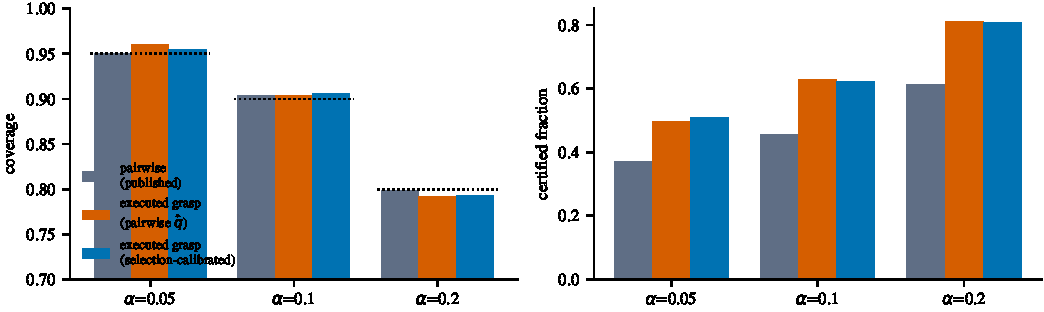
\includegraphics[width=\columnwidth]{figures/fig_selective_coverage.pdf}
\caption{Coverage and certified fraction for the executed grasp. Dotted lines mark the
target. Recalibrating on the selected action hits the target exactly and certifies more.}
\label{fig:selective}
\end{figure}

\section*{Conclusion}
\label{sec:conclusion}
We introduced an action-conditioned outcome bottleneck that transmits a compact stochastic interface without reconstructing geometry at deployment. One outcome model supports grasp selection, conformal filtering, active sensing, and latent adaptation; finite-probe theory characterizes local ambiguity, and split conformal provides marginal coverage for a randomized action under exchangeability.

On the evaluated simulator corpus, our model reaches 0.876 AUC and 0.984 success at 25\% commitment, versus 0.542 AUC and 0.503 selective success for Ferrari--Canny computed on an OBB reconstruction. These are controlled within-corpus comparisons, not evidence of superiority over true-geometry analytic metrics, matched-capacity learned scorers, uncertainty baselines, or rate-matched reconstruction, which remain unmeasured. The results support outcome-oriented compression as a promising hypothesis and identify those comparisons, physical deployment, and robust transfer as the next requirements.


\bibliographystyle{IEEEtran}
\bibliography{refs}

\end{document}
